%%%%%
\section{引言}

\begin{frame}{\secname}
\begin{itemize}
    \item “运筹于帷幄之中,决胜于千里之外”。运筹学将科学的方法、技术和工具应用到经济管理、工程设计等领域,以便为人们提供最佳的解决方案。
    \item 在这一章里,首先介绍运筹学的基本概况,包括运筹学的历史和发展,运筹学的性质和特点,运筹学研究的主要内容和以后的发展趋势。然后从运筹学问题解决过程的角度,依次介绍建模、求解和实际应用时应该注意的一些问题,使初学者对运筹学概念和方法有初步的认识。
\end{itemize}
\end{frame}

\subsection{运筹学概况}
\subsubsection{运筹学历史}
\begin{frame}[allowframebreaks]{\subsecname}
\begin{itemize}
    \item 运筹学的产生很难有一个明确的时间界定,目前国际上比较公认的观点是运筹学产生于第二次世界大战前后。
    \item 1937年英国部分科学家被邀请去帮助皇家空军研究雷达的部署和运作问题,目的在于最大限度地发挥有限雷达的效用,以应对德军的空袭。
    \item 1938年波德塞(Bawdsey)雷达站的负责人罗伊(Rowe)提出了优化防空作战系统运行的问题,并用“Operational Research”一词作为对这一方面研究的描述,这就是今天仍然将运筹学称为O.R.的历史由来。
    \item 1939年从事此方面问题研究的科学家被召集到英国皇家空军指挥总部,成立了一个由布莱开特(Blacket)领导的军事科技攻关小组;由于其成员学科性质的多样性,这一最早成立的军事科技攻关小组被戏称为“布莱开特马戏团”。由于“布莱开特马戏团”的活动是第一次有组织的系统的运筹学活动,所以后人将该小组的成立作为运筹学产生的标志。
    \item 此后,O.R.小组的活动范围不断扩大,从最初的仅限于空军,逐步扩展到了海军和陆军;研究内容也从对军事战术性问题的研究,逐步扩展到对军事战略性问题的研究。
    \item 由于科学家的天赋、战争的需要以及不同学科的交互作用,这一军事科技攻关小组在提高军事运筹水平方面取得了惊人的成功,这使得运筹学在整个军事领域迅速传播,到1941年英国皇家陆、海、空三军都成立了这样的科学小组。比较典型的论题包括雷达布置策略、反空袭系统控制、海军舰队的编制和对敌潜艇的探测等。
    \item 第二次大战结束以后,美国等国家的军方仍然保留了一些运筹小组,其他的多数人转向把运筹学研究应用于和平时期的工商业。因此美国,德国等国家的运筹学得以蓬勃发展,出现了应用研究和理论研究相互促进的局面。
    \item 从应用方面来讲,在工商业管理中的应用是主要的,特别是在美国,管理科学方面的主要内容便是运筹学。
    \item 从学校教育方面来说,许多大学理学院的数学系及工学院、管理学院、经济学院的许多系中都开设运筹学课程。
    \item 从科学发展来说,在运筹研究或运筹学这一名称下发展起来的分支学科就很多,如规划论(包含线性规划、非线性规划、整数规划、 动态规划、多目标规划等)、网络分析、排队论、对策论、决策论、存储论、可靠性理论、模型论、投入产出分析等等。
从学会方面来说,最早的是美国的运筹学会,成立于1952年。
\end{itemize}
\end{frame}

\subsubsection{运筹学的性质与特点}
\begin{frame}{\subsubsecname}
    运筹学是一门综合性应用型学科,也是上个世纪形成的一门科学。当人们把战时的运筹研究取得成功的经验在和平时期加以推广应用时,面临着一个广阔的研究领域。
\begin{itemize}
    \item 科学性:运筹学原理中引进了大量的数学研究方法。
\item 系统性:运筹学研究问题是从系统的观点出发,研究全局性的问题,研究综合优化的规律,它是系统工程的主要理论基础。
\item 应用性:在运筹学术界,有许多人强调运筹学的实用性和对研究结果的执行效果,并把执行效果看作运筹工作中的一个很重要的组成部分。
\item 跨学科性:
早期运筹学小组都是由不同领域的专家组成。
\item 理论和应用相互促进,相得益彰。
运筹学的各个分支学科,都是由于实际问题的需要或以一定的实际问题为背景逐渐发展起来的。
\end{itemize}
\end{frame}

\subsubsection{运筹学的主要内容}
\begin{frame}{\subsubsecname}
\begin{itemize}
    \item 运筹学的发展历史不算太长,但是其内容丰富,涉及面广,应用范围大,已经形成了一个相当庞大的学科。它的主要内容一般应该包含线性规划、非线性规划、整数规划、动态规划、多目标规划、随机规划、网络分析、排队论、对策论、 决策论、存储论、可靠性理论、模型论、投入产出分析等。它们中的每一部分都可以独立成册,都有丰富的内容。
    \item 上述的前六个部分统称为规划论,它们主要是解决两个方面的问题。一个方面的问题是对于给定的人力、物力和财力,怎样才能发挥他们的最大效益; 另一个方面的问题就是对于给定的任务,怎样才能用最少的人力、物力和财力去完成它。
\end{itemize}
\end{frame}

\subsection{运筹学问题的求解过程}
\begin{frame}{\subsecname}
    既然运筹学的使命是要解决问题,那么怎么样去解决呢?解决问题可以定义为:识别问题,确定备选方案,实施方案和评价方案这四个最基本的流程。那么运筹学问题的解决对应着从现实系统到模型,模型的求解,模型结论所提供的方案,现实结论以及实现效果。作为研究对象的系统来说,总是要求我们求解一定的未知量并给出相应的结论,求解过程如图\ref{fig:ch1-1}所示。图中虚线表示了人们最直接的目标,右侧的实线表示了这一目标的具体实现路径。
\begin{figure}[htbp]\label{fig:ch1-1}
  \centering
  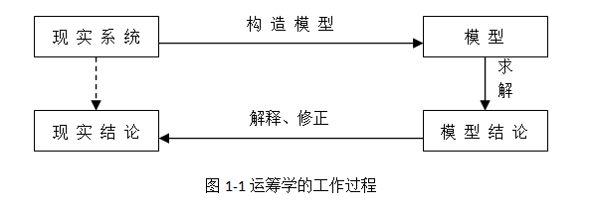
\includegraphics[width=5 in,height=2 in]{pic/1_1.png}
  \caption{运筹学的工作过程}
\end{figure}
\end{frame}

\subsubsection{从现实系统到理论模型:模型建立}
\begin{frame}[allowframebreaks]{\subsubsecname}
\begin{enumerate}
    \item 模型是现实世界的抽象化反映。运筹学的实质在于建立和使用模型来解决实际问题。尽管模型的具体结构和形式总是与要解决的问题相联系,但在这里将抛弃模型在外表上的差别,从最广泛的角度抽象出它们的共性。模型在某种意义上说是客观事物的简化与抽象,是研究者经过思维抽象后用文字、图表、符号、关系式以及实体模样对客观事物的描述。
    \item 模型有三种基本类型,即形象模型、模拟模型和数学模型。
\begin{itemize}
    \item 物理复制被称为形象模型,比如孩子的卡车,飞机模型等等。
\item 模拟模型也是物理模型,但是在外形上与被建模的对象并不一样,比如汽车上的速度表就是一种模拟模型。
\item 模型的第三种类型是数学模型,它是以一些系统化的符号和数学表达式或关系式来反映实际问题。
\end{itemize}
\item 运筹学模型主要是指数学模型。\\
数学模型可以简单的描述为:用字母、数字和运算符来精确地反映变量之间相互关系的式子或式子组。
数学模型由决策变量、约束条件和目标函数三个要素构成。决策变量即问题中所求的未知的量,约束条件是决策所面临的限制条件,目标函数则是衡量决策效益的数量指标。
一旦所有可控和非可控输入都已经确定,目标函数和约束条件就可在模型中被考虑,模型的输出便也确定下来。这样的话,模型的输出就是在那些实际环境因素和决策下会产生的结果了。图1-2表示的是数学模型如何将可控和非可控输入转化为结果输出以及这个生产模型的具体细节。

\begin{figure}\label{fig:ch1-2}
  \centering
  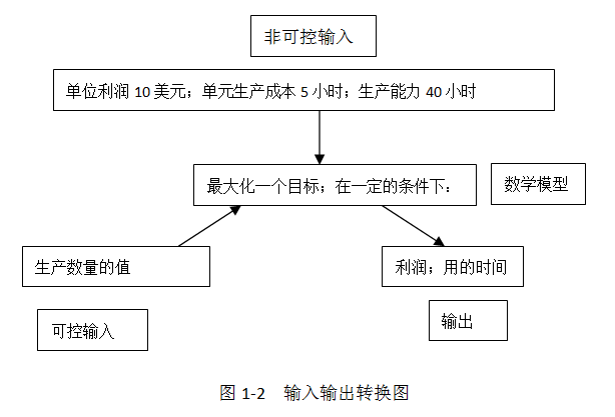
\includegraphics[width=4 in,height=3 in]{pic/1_2.png}
  \caption{}
\end{figure}
\begin{itemize}
    \item 非可控输入既可以是非常明确的,也可以是不确定的、变化的。
\item 如果一个模型的非可控输入都是已知的、不可变的,这样的模型称为确定模型。
\item 如果一个模型的非可控输入是不确定的、变化的,这样的模型就称为随机模型或概率模型。
\item 本书主要研究确定型数学模型。
\end{itemize}
\end{enumerate}
\end{frame}

\begin{frame}{\subsubsecname}
  了解模型的相关概念之后,下一个问题就是如何将一个现实问题转化为数学模型,也就是建模过程。既然运筹学模型的几个要素是:目标函数,约束条件(包括自然约束和强加约束),决策变量。那么根据我们要解决的问题,只要我们经常问自己下面这些问题,一个模型的框架是不难建立的。

\begin{itemize}
    \item 我们需要什么目标?
    \item 通过调节哪些因素可以使得我们达到这一目标?
    \item 调节的因素是变动的吗? 
    \item 要与实际情况相符合有什么限制条件吗?
     \item 在实现目标的过程中,有哪些约束条件?
      \item 这样建立的模型是相对完备的吗?
\end{itemize}

\end{frame}

\begin{frame}{\subsubsecname}
对以上问题的回答只是提供了一种建立模型的基本框架结果,对于数学规划类的建模,这种思路也是很有效的。一个问题解决的好坏,与建立的模型和所使用的工具关系是相当密切的。数学模型不可能完全刻画现实世界,正如经济学诺贝尔奖获得者和计算机图灵奖获得者,著名的决策理论专家所言,数学模型并不要求准确无误,它只需要尽可能接近地给出比靠常识得到更好的解就可以了。
\end{frame}

\subsubsection{模型到方案:模型的求解}
\begin{frame}{\subsubsecname}
    \begin{itemize}
        \item 一旦建模和数据准备工作已经完成,我们就可以进入模型求解阶段。在此阶段分析人员将确定决策变量的具体值,以获得模型的最优输出结果。这些具体的决策变量的值,或者说能够得到最优输出结果的值,通常称为模型的最优解。对于前面的生产问题来说,模型的求解阶段包括,找到能实现最大化利润,同时又不违反生产能力约束条件的决策变量(生产数量)的值。
\item 模型求解的过程中可能会用到一种反复实验的方法。通过对提供的一些备选方案进行测试评估,可以得到满足条件的较好方案。如果某个方案不能满足其中的一个或多个约束条件,那么无论目标函数的值是多少,这个方案都是不可行的,从而不能被采纳。如果所有的约束条件都满足了,那么它就是可行解,或者说是备选项。
\item 整个运筹学的学习,就是要有效率地解决问题,模型和算法的好坏直接影响了这一目标的实现。对于算法的设计,方法有很多,在我们运筹学的学习中,主要是强调迭代法。尽管问题千差万别,但是具体的步骤却是差不多的。为了更形象的说明这一步骤,我们不妨举个例子。你现在要到一个地方。这个时候你可能会考虑以下几个问题:
\begin{itemize}
    \item (1)我现在在哪里?
\item (2)我将要去哪里?
\item (3)朝哪个方向走?
\item (4)选择每步走多大的一步?
\end{itemize}
    \end{itemize}
\end{frame}

\begin{frame}{\subsubsecname}
一个迭代算法的思想和我们要去一个地方这一目标的思想是一致的。在设计一个迭代算法的时候,我们依然是考虑这四个问题。迭代算法主要就是通过当前点到下一个点的变化来实现。先找到当前点,这是我们的新的起点,然后通过一定的规则到达下一个点,以下一个点为当前点,继续后面的过程直至终止。对应上面四个问题,我们考虑的是:
\begin{itemize}
\item (1)初始点(我现在在哪里);
\item (2)终止准则(我们的目标是什么);
\item (3)迭代方向(朝哪个方向走);
\item (4)迭代步长(选择每步都多远)。
\end{itemize}
\end{frame}

\subsubsection{从结果到结论}
\begin{frame}{\subsubsecname}
   通过计算机或者手工得到的最优解不一定我们需要的结论。通过定量计算求解只是决策的一部分工作,还不是作为管理者和决策者要的结论。决策者需要的是可以具体实施的简单易行的报告。报告除了推荐的方案和一些有助于决策的相关信息,所推荐的方案不仅在理论上能够说服别人,在实践上也是简单可行的。所以在使用软件的同时,更重要的是能够正确的解读软件给我们的结果。在具体的问题中,我们将继续探讨这一问题。
\end{frame}



\begin{frame}{矩阵表示}
$$
\begin{gathered}
    \begin{matrix}
    0&1 \\ 1&0
    \end{matrix}
    \quad
    \begin{pmatrix}
    0 &-i \\ i &0
    \end{pmatrix}
    \quad
    \begin{bmatrix}
    0 & -1\\1&0
    \end{bmatrix}
\end{gathered}
$$
\end{frame}